%!TEX program = xelatex
\documentclass[10pt]{beamer}
\usepackage{graphicx}
\usepackage{booktabs}
\linespread{1.11}
\usepackage{tikz}
\tikzset{global scale/.style={
    scale=#1,
    every node/.style={scale=#1}
  }
}
\setcounter{tocdepth}{1}

\usetheme[menuwidth={0.5\paperwidth}]{erlangen}
\setbeamercovered{transparent=20}
\setbeamerfont{frametitle}{series=\bfseries}
\usepackage{hyperref}
\hypersetup{colorlinks=false,
            colorlinks=black,
            pdfborder=100,
            citecolor=black}


\setbeamerfont{block title}{series=\bfseries}
\usepackage{graphicx}
\setbeamerfont{myTOC}{series=\bfseries}
\AtBeginSection[]{\frame{\frametitle{Current Section}%
                  \usebeamerfont{myTOC}\tableofcontents[current]}}

\usepackage[no-math,cm-default]{fontspec}
\setmainfont{Minion Pro}
\setsansfont[BoldFont={Myriad Pro Semibold}]{Myriad Pro}
\setmonofont{Courier New}
\usepackage{xeCJK}
\setCJKmainfont[BoldFont={方正黑体简体},ItalicFont={楷体}]{宋体}
\setCJKsansfont[BoldFont={方正黑体简体}]{方正中等线简体}
\setCJKmonofont{方正中等线简体}
\XeTeXlinebreaklocale "zh"
\XeTeXlinebreakskip = 0pt plus 1pt

\usefonttheme[onlymath]{serif}
\usepackage[noamssymbols]{mtpro2}

% \renewcommand\contentsname{目录}
\setbeamertemplate{itemize items}{\raisebox{0.15ex}{\small$\bullet$}}

\begin{document}
\title{Business Cycles and the Asset Structure of Foreign Trade}
\subtitle{(IER, 1995)}
\author{Marianne Baxter, Mario J. Crucini}

\date{\today}
% \institute{The School of Economics\\
  % \vspace{-0.2em}{\small Fudan University} }

\begin{frame}[plain]
  \titlepage
\end{frame}

%%%%%%%%%%%%%%%%%%%%%%%%%%%%%%%%%%%%%%%%%%%%%%%%%%%%%%
%%%%%%%%%%%%%%%%%%%%%%%%%%%%%%%%%%%%%%%%%%%%%%%%%%%%%%
\begin{frame}{Contents}
\tableofcontents
\end{frame}

%%%%%%%%%%%%%%%%%%%%%%%%%%%%%%%%%%%%%%%%%%%%%%%%%%%%%%
%%%%%%%%%%%%%%%%%%%%%%%%%%%%%%%%%%%%%%%%%%%%%%%%%%%%%%
\section{Introduction}
\begin{frame}{Motivation}
\begin{enumerate}
  \item \textbf{Reason}: The extent of international \alert{financial integration} is important for international \alert{business cycles}.
\begin{itemize}
  \item Individuals' incentive to \alert{smooth consumption} in response to fluctuations in income via financial markets.
  \item The extent to which a country can trade on world financial markets will determine the extent to which its citizens can \alert{insure} themselves against nation-specific components of \alert{business-cycle risk}.
\end{itemize}
  \item \textbf{Goal}: To provide a detailed analysis of the channels through which international financial linkages affect international business cycles.
\end{enumerate}
\end{frame}

\section{Model}
\begin{frame}{Preferences}
\begin{itemize}
  \item Preferences:
  \begin{eqnarray}
  &&\mathbb{E}_0\sum_{t=0}^{\infty}{\beta}^t \frac{1}{1-\sigma} [C_t^\theta L_t^{1-\theta}]^{1-\sigma}, \quad \text{home country;}\\
  &&\mathbb{E}_0\sum_{t=0}^{\infty}{\beta}^t \frac{1}{1-\sigma} [(C_t^*)^\theta (L_t^*)^{1-\theta}]^{1-\sigma},\quad \text{foreign country.}
  \end{eqnarray}
  \item Time Constraints:
  \begin{align}
  1-L_t-N_t &\geq  0,\quad \text{home country;}\\
  1-L_t^*-N_t^* & \geq  0,\quad \text{foreign country.}
  \end{align}
\end{itemize}
\end{frame}

\begin{frame}{Technology}
\begin{itemize}
  \item Production Function:
  \begin{align}
  Y_t &= A_t K_t^{1-\alpha}(X_tN_t)^\alpha,\quad \text{home country;} \\
  Y_t^* &= A_t^* (K_t^*)^{1-\alpha_*}(X_t^*N_t^*)^{\alpha_*},\quad \text{foreign country.}
  \end{align}
  where $X_t$ and $X_t^*$ are purely \alert{labor-augmenting} technical change in the home and foreign countries, and grow at a common, constant gross rate: $\gamma=X_{t+1}/X_t=X_{t+1}^*/X_t^*$.
  \item Capital Accumulations:
  \begin{align}
  K_{t+1}&=(1-\delta)K_t+\phi(I_t/K_t)K_t,\quad \text{home country;} \\
  K_{t+1}^*&=(1-\delta)K_t^*+\phi(I_t^*/K_t^*)K_t^*, \quad \text{foreign country.}
  \end{align}
\end{itemize}
\end{frame}

\begin{frame}{Complete Markets}
\begin{itemize}
    \item Social Planner's Problem
\begin{eqnarray*}
\max \mathcal{L}&=&\mathbb{E}_0 \sum_{t=0}^{\infty}\tilde{\beta}^t \{[\pi u(c_t,L_t)+(1-\pi)u(c_t^*,L_t^*)]\\
&&+ \pi w_t(1-L_t-N_t)+(1-\pi)w_t^*(1-L_t^*-N_t^*) \\
&&+\pi \lambda_t [(1-\delta)k_t-(\gamma k_{t+1}-\phi(i_t/k_t)k_t)] \\
&&+(1-\pi)\lambda_t^*[(1-\delta)k_t^*-(\gamma k_{t+1}^*-\phi(i_t^*/k_t^*)k_t^*)] \\
&&+p_t[\pi(A_tF(k_t,N_t)-c_t-i_t) \\
&&+(1-\pi)(A_t^*F(k_t^*,N_t^*)-c_t^*-i_t^*)]\}
\end{eqnarray*}
\item where $\tilde{\beta} \equiv \beta\gamma^{\theta(1-\sigma)}$, the multipliers are interpreted as:
\begin{itemize}
  \item $w_t,w_t^*$: wage rate
  \item $\lambda_t,\lambda_t^*$: price of existing capital
  \item $p_t$: price of the final good(price of new capital)
\end{itemize}
\end{itemize}


\end{frame}

\begin{frame}{Complete Markets}
FOCs:
\begin{small}
\begin{eqnarray}
&&c_t:p_t=u_1(c_t,L_t)\\
&&L_t:w_t=u_2(c_t,L_t)\\
&&N_t:w_t=p_tA_tF_2(k_t,N_t) \\
&&i_t:p_t=\lambda_t \phi'(i_t/k_t) \\
&&k_{t+1}:\gamma\lambda_t=E_t \mu(\frac{i_{t+1}}{k_{t+1}})\tilde{\beta}\lambda_{t+1}+\tilde{\beta}E_tp_{t+1}A_{t+1}F_1(k_{t+1},N_{t+1})\\
&&w_t:1-L_t-N_t=0 \\
&&\lambda_t:\gamma k_{t+1}=(1-\delta)k_t+\phi(i_t/k_t)k_t \\
&&p_t:\pi[y_t-c_t-i_t]+(1-\pi)[y_t^*-c_t^*-i_t^*]=0
\end{eqnarray}
\end{small}
where $\mu(z)\equiv [\phi(z)-z\phi_1(z)+(1-\delta)]$.
\end{frame}

\begin{frame}{Small Open Economy: Partial Equilibrium}
\begin{itemize}
    \item The economy is too small to affect the world interest rate. Flow budget constraint: . ($P_t^B \equiv (1+r_t)^{-1}$)
\begin{equation}
    \gamma P_t^Bb_{t+1}+c_t+i_t \leq y_t+b_t
\end{equation}
\begin{eqnarray*}
\max \mathcal{L}&=&\mathbb{E}_0 \sum_{t=0}^{\infty}\tilde{\beta}^t \{u(c_t,L_t)+w_t(1-L_t-N_t)\\
&&+\lambda_t[(1-\delta)k_t-(\gamma k_{t+1}-\phi(i_t/k_t)/k_t)]\\
&&+p_t(y_t+b_t-\gamma P_t^Bb_{t+1}-c_t-i_t)\}
\end{eqnarray*}
\item Additional FOCs:
\begin{eqnarray}
&&b_{t+1}:\tilde{\beta}E_tp_{t+1}-\gamma p_tP_t^B=0 \\
&&p_t:b_t+A_tF(k_t,N_t)-c_t-i_t-\gamma P_t^Bb_{t+1}=0
\end{eqnarray}
\item  Transversality Conditions:
\begin{align}
\mathop {\lim }\limits_{t \to \infty }\tilde{\beta}^tp_tb_{t+1}&=0
% \mathop {\lim }\limits_{t \to \infty }\tilde{\beta}^tp_t^{*}b_{t+1}^{*}&=0
\end{align}
\end{itemize}

\end{frame}

\begin{frame}{General Equilibrium with Restricted Asset Markets}
\begin{itemize}
    \item Each country can trade a noncontingent real bond with residents of the other country. The interest rate adjusts to clear the bond market. Bond-market clearing condition:
\begin{eqnarray}
\pi b_t+(1-\pi)b_t^*=0
\end{eqnarray}
    \item Aggregate financial asset accumulation satisfies:
\begin{align}
\gamma\pi P_t^Bb_{t+1}+\gamma(1-\pi)P_t^Bb_{t+1}^* &\leq\nonumber \\
\pi[b_t+y_t-c_t-i_t]&+(1-\pi)[b_t^*+y_t^*-c_t^*-i_t^*]
\end{align}
which implies
\begin{eqnarray}
\pi(A_tF(k_t,N_t)-i_t-c_t)+(1-\pi)(A_t^*F(k_t^*,N_t^*)-c_t^*-i_t^*)\geq 0
\end{eqnarray}
\end{itemize}



\end{frame}

\begin{frame}{General Equilibrium with Restricted Asset Markets}
\begin{itemize}
\item FOCs:
\begin{eqnarray}
&&b_{t+1}:\tilde{\beta}E_tp_{t+1}-\gamma p_tP_t^B=0 \\
&&b_{t+1}^*:\tilde{\beta}E_tp_{t+1}^*-\gamma p_t^*P_t^B=0 \\
&&p_t:b_t+A_tF(k_t,N_t)-c_t-i_t-\gamma P_t^Bb_{t+1}=0\\
&&p_t:b_t^*+A_t^*F(k_t^*,N_t^*)-c_t^*-i_t^*-\gamma P_t^Bb_{t+1}^*=0
\end{eqnarray}
\item The interest rate is endogenously determined:
\begin{eqnarray*}
P_t^B=\tilde{\beta}E_t(p_{t+1}/\gamma p_t)=\tilde{\beta}E_t(p_{t+1}^*/\gamma p_t^*)
\end{eqnarray*}
\end{itemize}

\end{frame}

\section[Implications]{Implications for Business Cycles}
\begin{frame}{Business Cycle Statistics}
\begin{figure}[thbp]
  \centering
  
\includegraphics[width=0.90\textwidth]{1.png}
\end{figure}
\end{frame}

\begin{frame}{Calibration}
\begin{figure}[thbp]
  \centering
  
\includegraphics[width=0.90\textwidth]{2.png}
\end{figure}
\end{frame}

\begin{frame}{BKK's Productivity Shocks Process}
\begin{equation*}
\begin{bmatrix}
\log A_{t}\\
\log A_{t}^{*}
\end{bmatrix}
= \begin{bmatrix}
\rho & \nu\\
\nu^{*} & \rho^{*}
\end{bmatrix}
\begin{bmatrix}
\log A_{t-1}\\
\log A_{t-1}^{*}
\end{bmatrix}
+ \begin{bmatrix}
\epsilon_{t}\\
\epsilon_{t}^{*}
\end{bmatrix}
\end{equation*}

\begin{figure}[thbp]
  \centering
  
\includegraphics[width=0.75\textwidth]{3.png}
\end{figure}
\begin{itemize}
  \item Shocks to productivity are \alert{highly persistent}, and there is some \alert{evidence of transmission} of shocks from one country to another.
  \item The innovations to productivity are \alert{positively correlated} across countries.
\end{itemize}
\end{frame}

\begin{frame}{Unit Root Test}
$H_0$: The Solow residuals follow a random walk without spillovers, but with possibly correlated innovations. $\Rightarrow$ Fail to reject.
\begin{figure}[thbp]
  \centering
  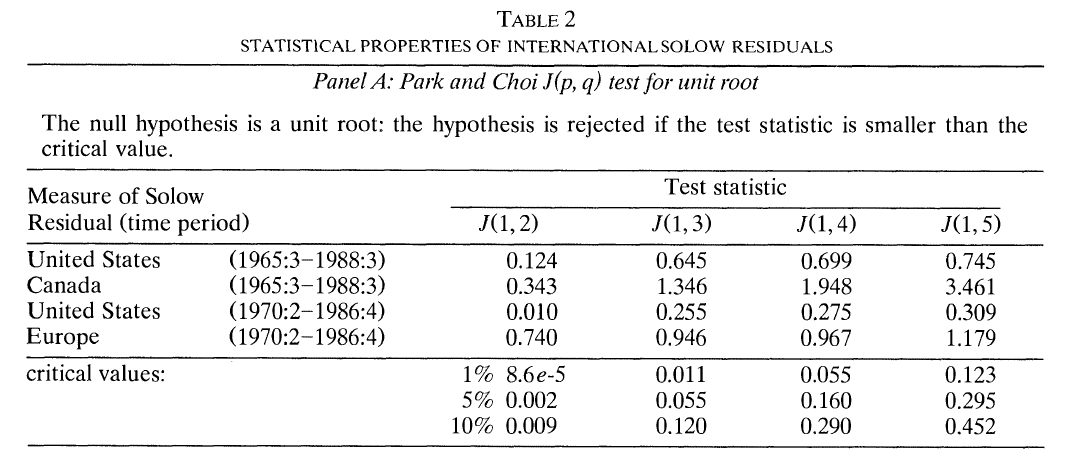
\includegraphics[width=0.90\textwidth]{4.png}
\end{figure}
\end{frame}

\begin{frame}{Cointegration Tests}
\begin{figure}[thbp]
  \centering
  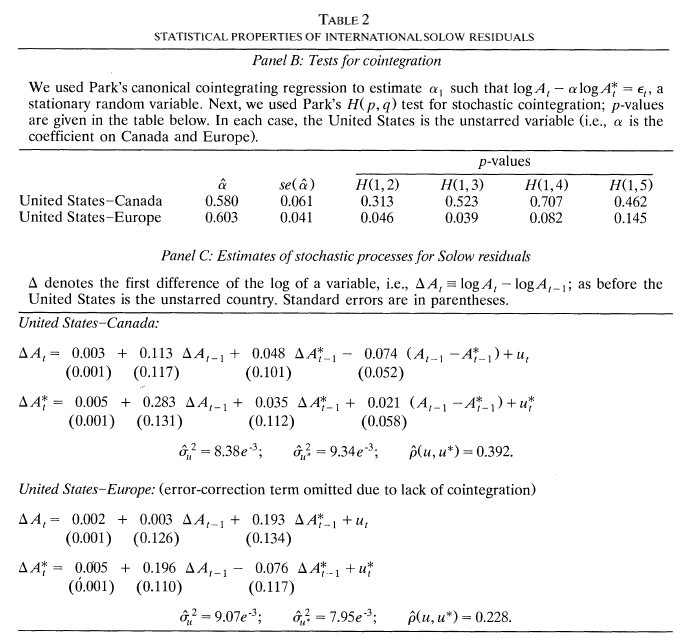
\includegraphics[width=0.75\textwidth]{5.png}
\end{figure}
%\begin{itemize}
%  \item No significant international transmission of shocks, with the possible exception of transmission between the United States and Canada.
%  \item Cannot reject the hypothesis that productivity in each country follows a random walk with drift, without transmission, but with innovations that are positively correlated across countries.
%\end{itemize}
\end{frame}

\begin{frame}{Trend Stationary Productivity with Spillovers}
$\rho=\rho^*=0.906$, $\nu=\nu^*=0.088$, $\rho(\epsilon_t,\epsilon_t^*)=0.258$.
\begin{figure}[thbp]
  \centering
  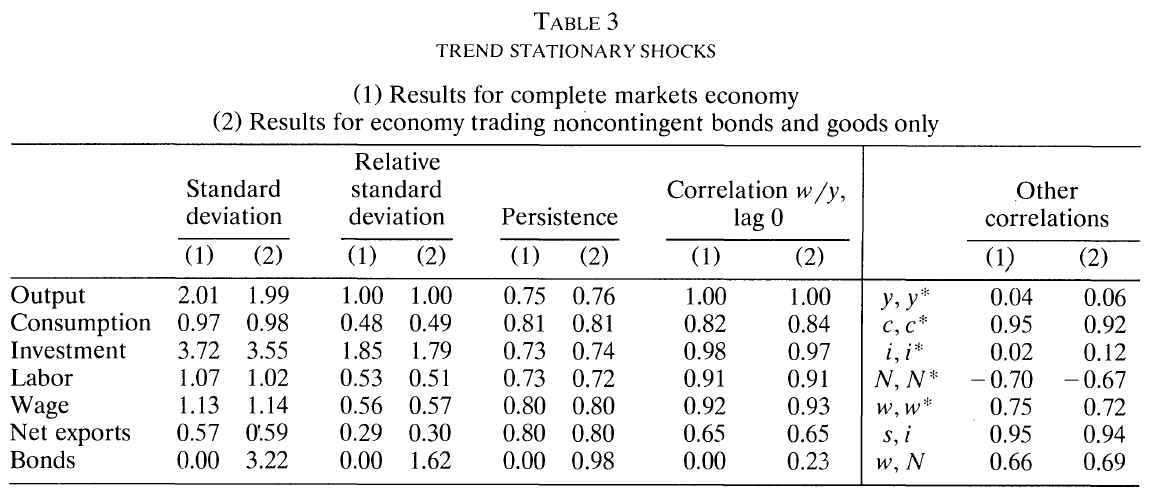
\includegraphics[width=0.90\textwidth]{6.png}
\end{figure}
%\begin{footnotesize}
%\begin{itemize}
%  \item high international consumption correlations
%  \item negative international correlations of output, labor input and investment
%  \item a strong persistent correlation between labor input and real wages
%\end{itemize}
%\end{footnotesize}
\end{frame}

\begin{frame}{Random-Walk Productivity without Spillovers}
$\rho=\rho^*=1$, $\nu=\nu^*=0$.
\begin{figure}[thbp]
  \centering
  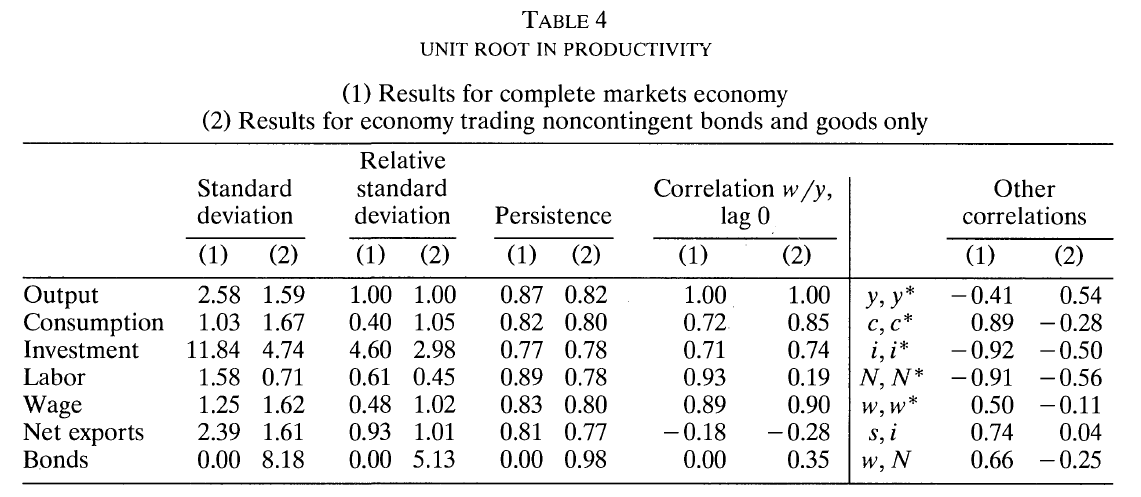
\includegraphics[width=0.90\textwidth]{7.png}
\end{figure}
%\begin{footnotesize}
%\begin{itemize}
%  \item higher volatility of output, investment and labor input in complete markets case
%  \item \textit{positive} international output correlation and \textit{negative} consumption correlation under bond economy.
%  \item weaker contemporaneous correlation of labor in bond economy; positive(negative) correlation between productivity and labor input in complete(restricted) markets case.
%\end{itemize}
%\end{footnotesize}
\end{frame}

\begin{frame}{Cross-Country Correlation v.s. Persistence}
\begin{columns}
\begin{column}{0.49\paperwidth}
\begin{figure}[thbp]
  \centering
  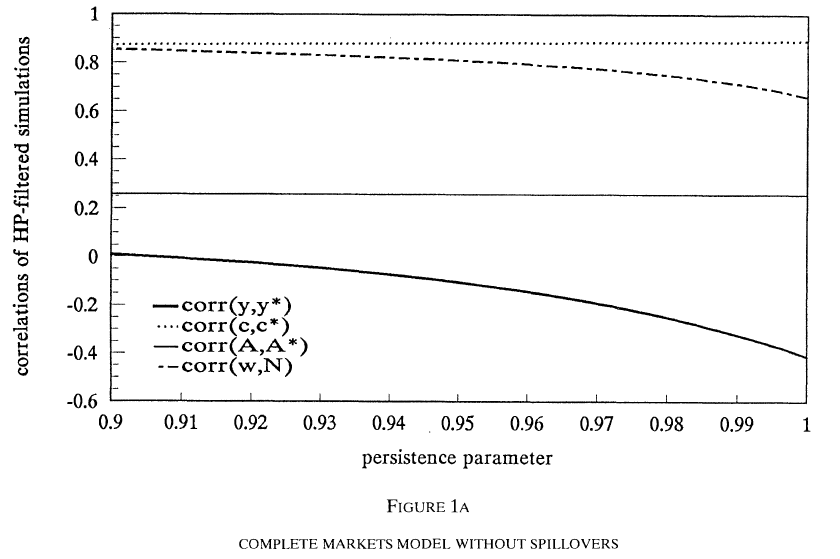
\includegraphics[width=0.90\textwidth,height=0.5\textheight]{8.png}
\end{figure}
\end{column}

\begin{column}{0.49\paperwidth}
\begin{figure}[thbp]
  \centering
  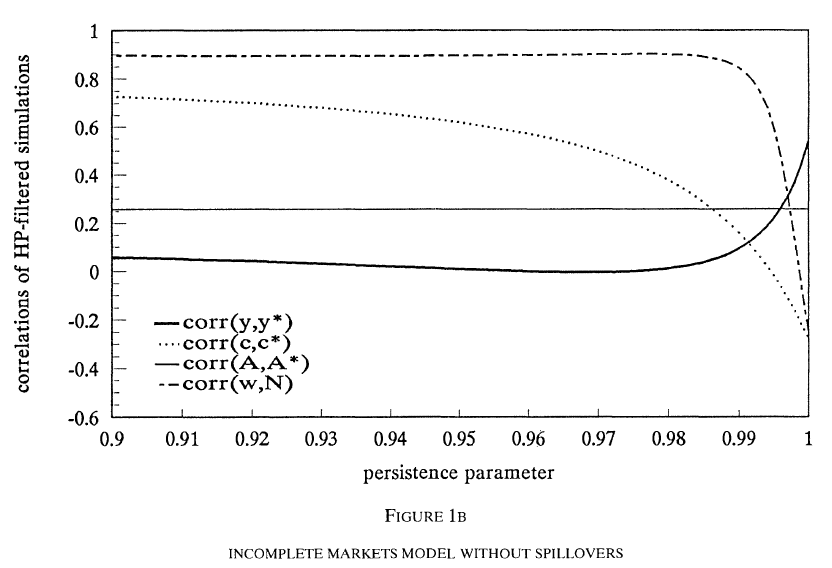
\includegraphics[width=0.90\textwidth,height=0.5\textheight]{9.png}
\end{figure}
\end{column}
\end{columns}
\end{frame}

\section[Dynamic Analysis]{Dynamic Response to a Productivity Shock}

% \begin{frame}{Trend-Stationary Shocks with Spillovers}
% \begin{figure}[thbp]
%   \centering
%   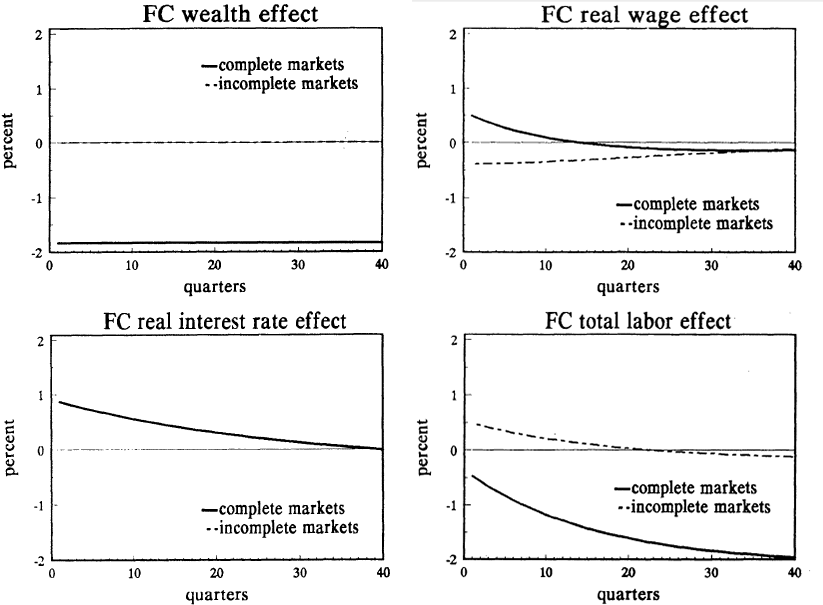
\includegraphics[width=0.90\textwidth]{16.png}
% \end{figure}
% \end{frame}

\begin{frame}{Trend-Stationary Shocks with Spillovers}
\begin{figure}[thbp]
  \centering
  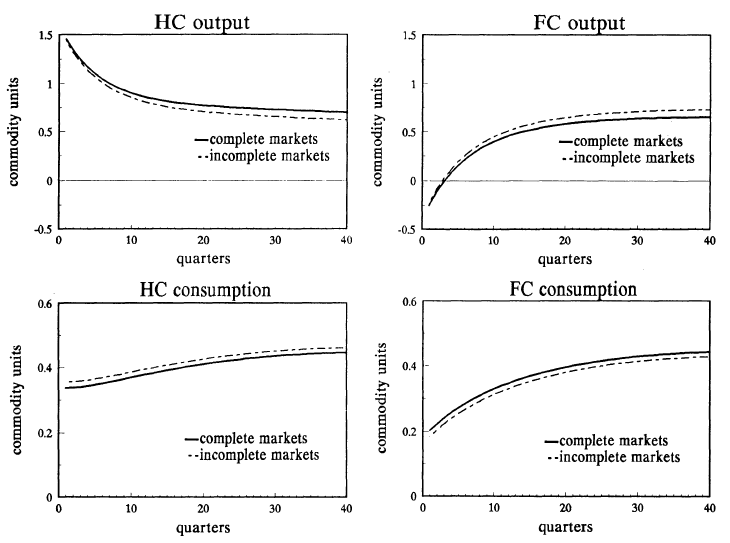
\includegraphics[width=0.90\textwidth]{17.png}
\end{figure}
\end{frame}

\begin{frame}{Trend-Stationary Shocks with Spillovers}
\begin{figure}[thbp]
  \centering
  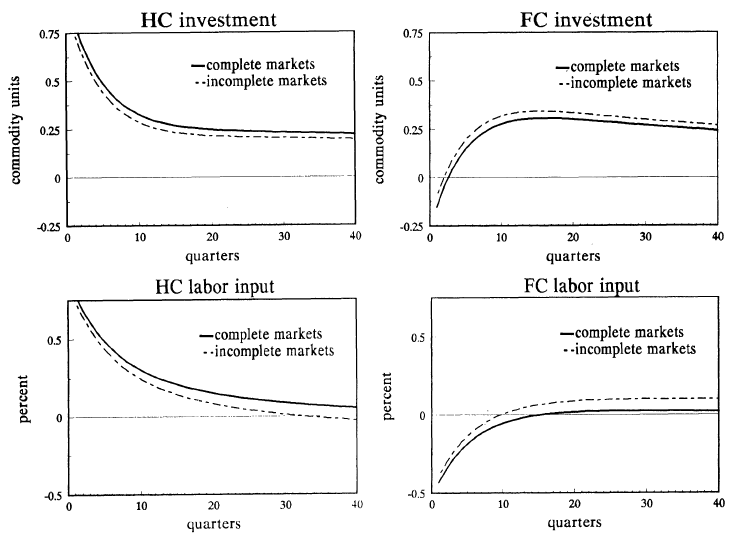
\includegraphics[width=0.90\textwidth]{18.png}
\end{figure}
\end{frame}

\begin{frame}{Trend-Stationary Shocks with Spillovers}
\begin{figure}[thbp]
  \centering
  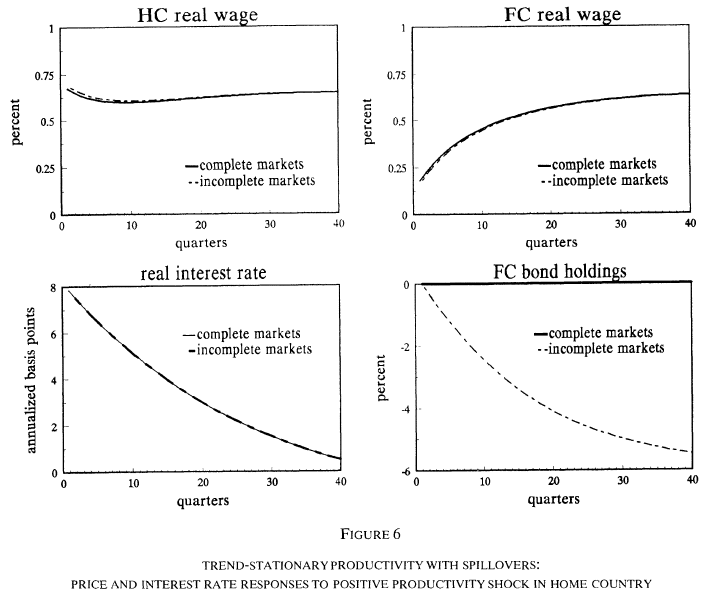
\includegraphics[width=0.85\textwidth]{19.png}
\end{figure}
\end{frame}

\begin{frame}{Trend-Stationary Shocks with Spillovers}
\begin{figure}[thbp]
  \centering
  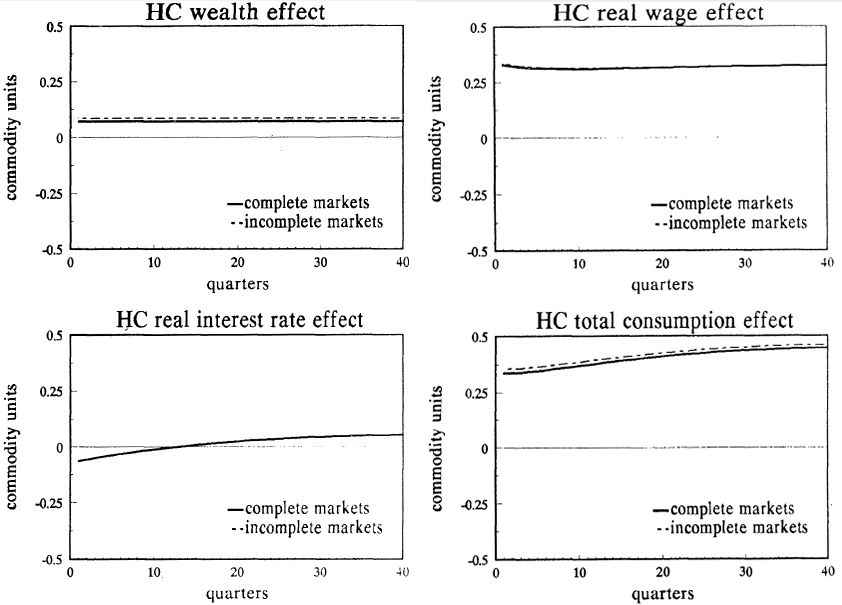
\includegraphics[width=0.90\textwidth]{20.png}
\end{figure}
\end{frame}

\begin{frame}{Trend-Stationary Shocks with Spillovers}
\begin{figure}[thbp]
  \centering
  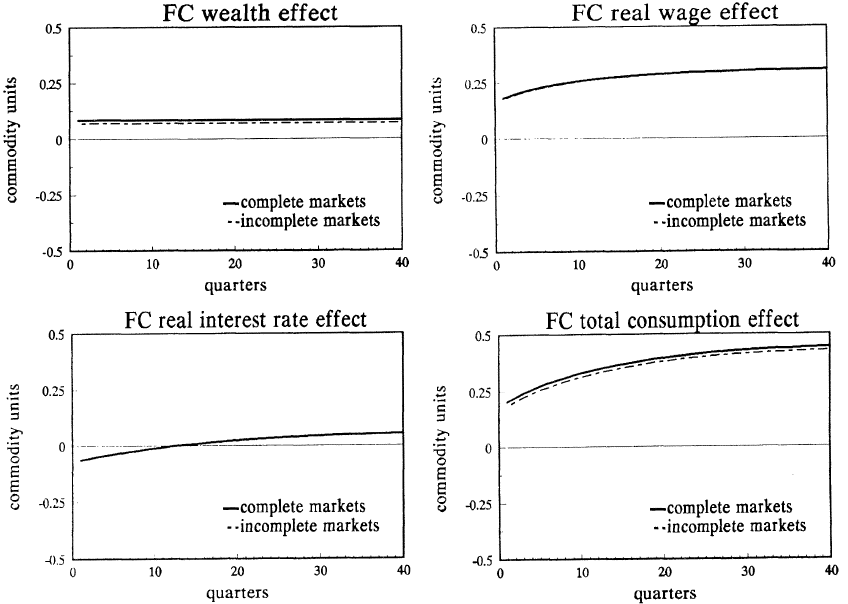
\includegraphics[width=0.90\textwidth]{21.png}
\end{figure}
\end{frame}

\begin{frame}{Trend-Stationary Shocks with Spillovers}
\begin{figure}[thbp]
  \centering
  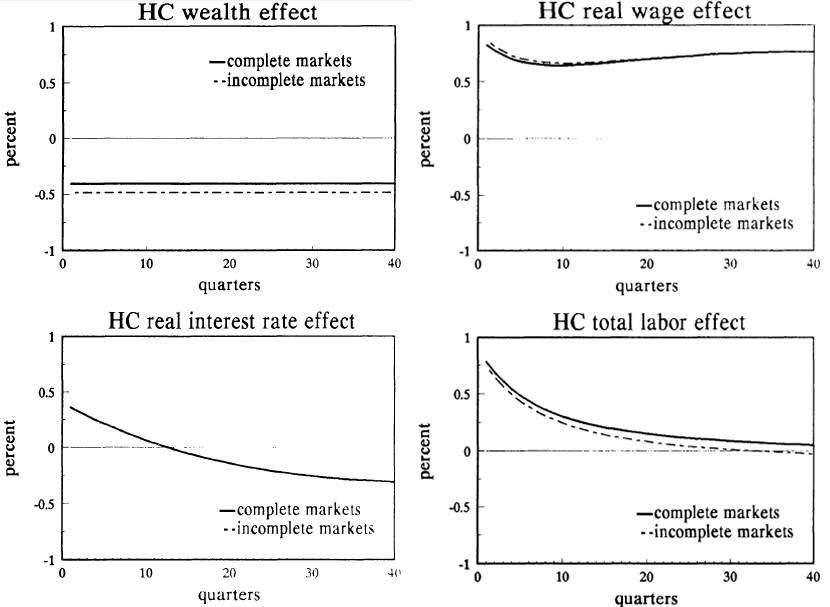
\includegraphics[width=0.90\textwidth]{22.png}
\end{figure}
\end{frame}

\begin{frame}{Trend-Stationary Shocks with Spillovers}
\begin{figure}[thbp]
  \centering
  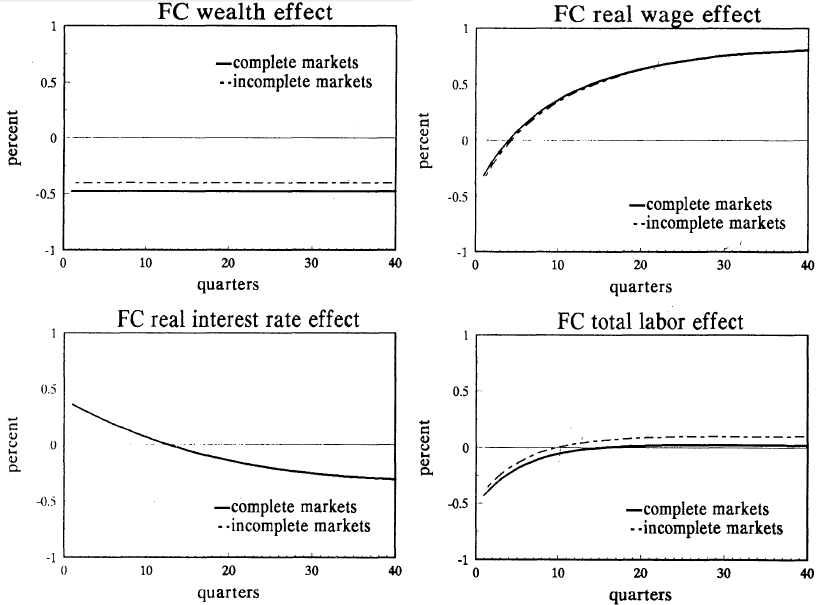
\includegraphics[width=0.90\textwidth]{23.png}
\end{figure}
\end{frame}



\begin{frame}{Random Walk Productivity}
\begin{figure}[thbp]
  \centering
  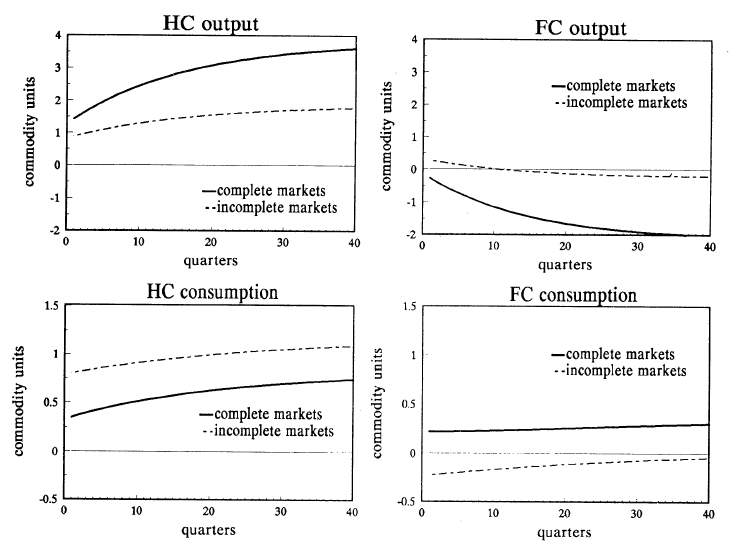
\includegraphics[width=0.90\textwidth]{10.png}
\end{figure}
\end{frame}

\begin{frame}{Random Walk Productivity}
\begin{figure}[thbp]
  \centering
  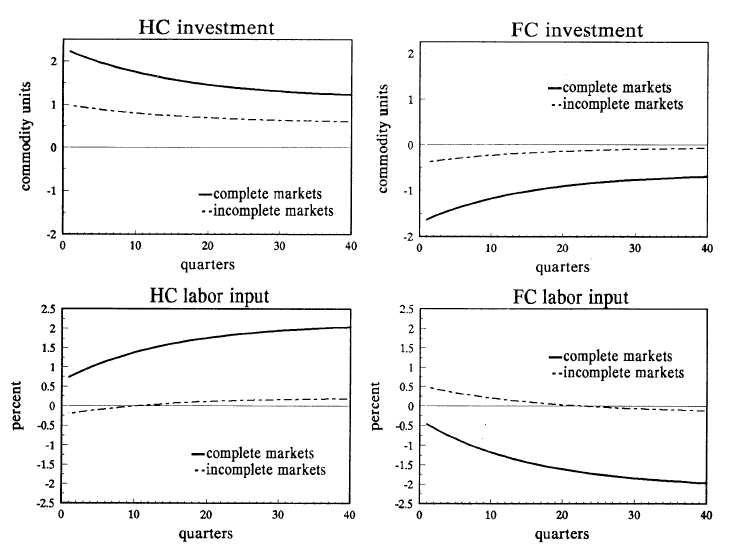
\includegraphics[width=0.90\textwidth]{11.png}
\end{figure}
\end{frame}

\begin{frame}{Random Walk Productivity}
\begin{figure}[thbp]
  \centering
  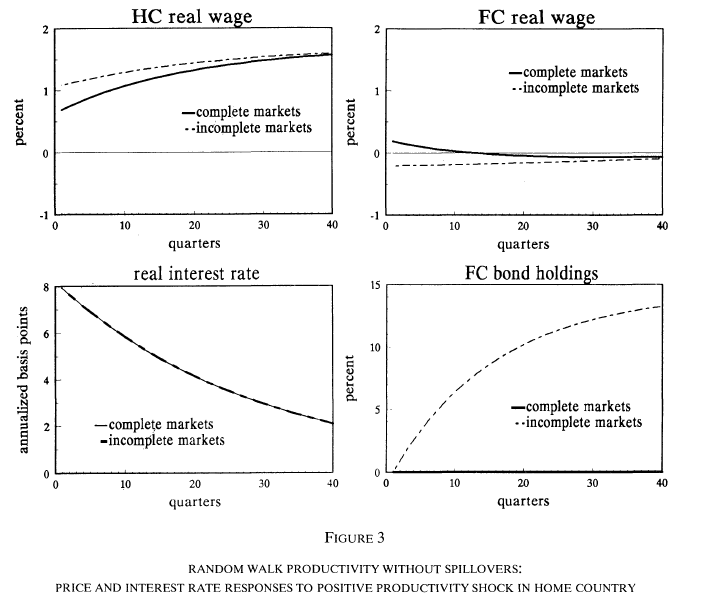
\includegraphics[width=0.85\textwidth]{12.png}
\end{figure}
\end{frame}

\begin{frame}{Random Walk Productivity}
\begin{figure}[thbp]
  \centering
  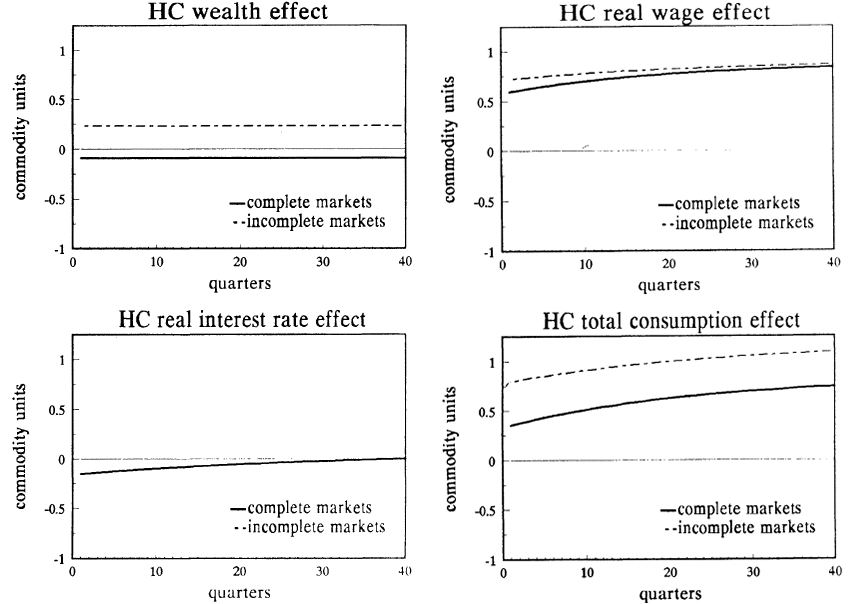
\includegraphics[width=0.90\textwidth]{13.png}
\end{figure}
\end{frame}

\begin{frame}{Random Walk Productivity}
\begin{figure}[thbp]
  \centering
  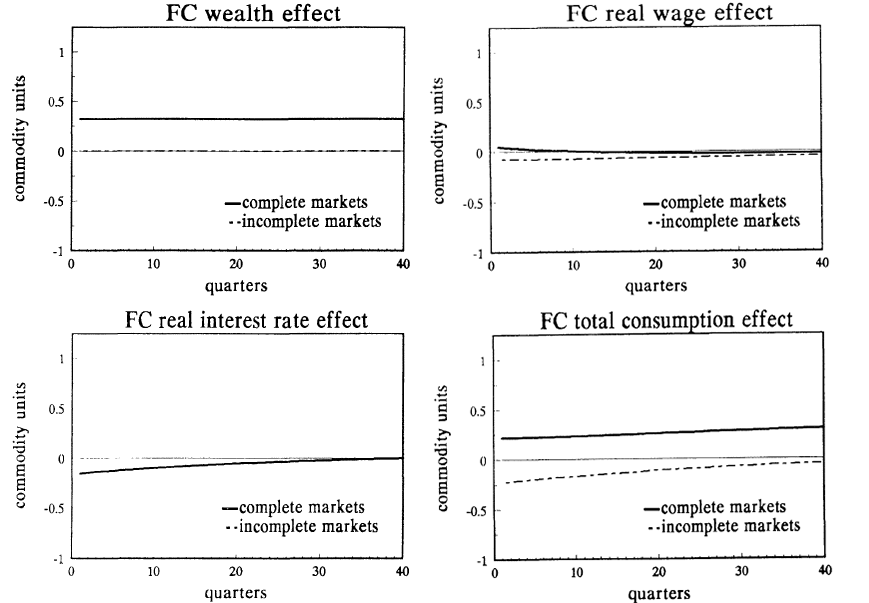
\includegraphics[width=0.90\textwidth]{14.png}
\end{figure}
\end{frame}

\begin{frame}{Random Walk Productivity}
\begin{figure}[thbp]
  \centering
  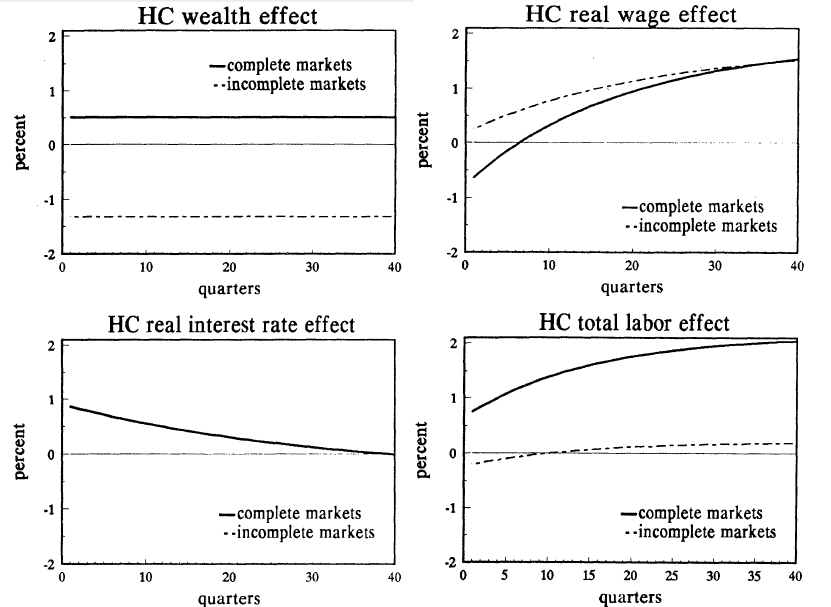
\includegraphics[width=0.90\textwidth]{15.png}
\end{figure}
\end{frame}

\begin{frame}{Random Walk Productivity}
\begin{figure}[thbp]
  \centering
  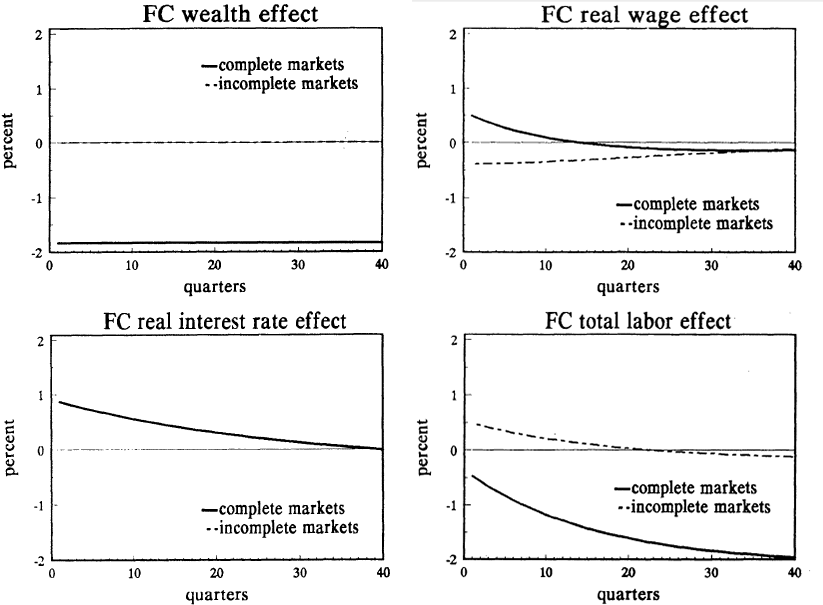
\includegraphics[width=0.90\textwidth]{16.png}
\end{figure}
\end{frame}



\section{Conclusion}

\begin{frame}{Crucial Findings}
\begin{enumerate}
  \item Incomplete Markets v.s. Complete Markets model
  \begin{itemize}
    \item Trend stationary international productivity process with substantial international "spillovers" of productivity shocks, \alert{indistinguishable}.
    \item Productivity in each country follows a random walk without spillovers but with correlated innovations, \alert{quite different}.
  \end{itemize}
  \item Major differences in the macroeconomic response to shocks under the alternative asset structures are due almost entirely to differential wealth effects.
  \item Incomplete markets with random-walk productivity specification can generate results which are closer to data.
\end{enumerate}
\end{frame}

\end{document}
